\documentclass[12pt]{book}

\title{Think Go}
\author{Luciano Ramalho, Allen B. Downey, and Chris Mayfield}

\newcommand{\thetitle}{Think Go}
\newcommand{\thesubtitle}{How to Think Like a Computer Scientist}
\newcommand{\theauthors}{Luciano Ramalho, Allen B. Downey, and Chris Mayfield}
\newcommand{\theversion}{0.1.0}

%%%% Both LATEX and PLASTEX

\usepackage{graphicx}
\usepackage{setspace}

%BEGIN LATEX
\usepackage{comment}
\excludecomment{htmlonly}
\includecomment{latexonly}

\usepackage{imakeidx}
\makeindex[options= -s headings.ist]
%END LATEX

% automatically index glossary terms
\newcommand{\term}[1]{%
\item[#1:]\index{#1}}

\usepackage{amsmath}
\usepackage{amsthm}

% format end of chapter excercises
\newtheoremstyle{exercise}
  {12pt}        % space above
  {12pt}        % space below
  {}            % body font
  {}            % indent amount
  {\bfseries}   % head font
  {}            % punctuation
  {12pt}        % head space
  {}            % custom head
\theoremstyle{exercise}
\newtheorem{exercise}{Exercise}[chapter]

\newif\ifplastex
\plastexfalse

%%%% PLASTEX ONLY
\ifplastex

\usepackage{localdef}

\usepackage{url}

\newcount\anchorcnt
\newcommand*{\Anchor}[1]{%
  \@bsphack%
    \Hy@GlobalStepCount\anchorcnt%
    \edef\@currentHref{anchor.\the\anchorcnt}%
    \Hy@raisedlink{\hyper@anchorstart{\@currentHref}\hyper@anchorend}%
    \M@gettitle{}\label{#1}%
    \@esphack%
}

% code listing environments:
% we don't need these for plastex because they get replaced
% by preprocess.py
%\newenvironment{code}{\begin{verbatim}}{\end{verbatim}}
%\newenvironment{stdout}{\begin{verbatim}}{\end{verbatim}}

% inline syntax formatting
\newcommand{\java}{\verb}%}

%%%% LATEX ONLY
\else

\sloppy
%\setlength{\topmargin}{-0.375in}
%\setlength{\oddsidemargin}{0.0in}
%\setlength{\evensidemargin}{0.0in}

% Uncomment these to center on 8.5 x 11
%\setlength{\topmargin}{0.625in}
%\setlength{\oddsidemargin}{0.875in}
%\setlength{\evensidemargin}{0.875in}

%\setlength{\textheight}{7.2in}

\setlength{\headsep}{3ex}
\setlength{\parindent}{0.0in}
\setlength{\parskip}{1.7ex plus 0.5ex minus 0.5ex}
\renewcommand{\baselinestretch}{1.02}

% see LaTeX Companion page 62
\setlength{\topsep}{-0.0\parskip}
\setlength{\partopsep}{-0.5\parskip}
\setlength{\itemindent}{0.0in}
\setlength{\listparindent}{0.0in}

% see LaTeX Companion page 26
% these are copied from /usr/local/teTeX/share/texmf/tex/latex/base/book.cls
% all I changed is afterskip

\makeatletter

\renewcommand{\section}{\@startsection 
    {section} {1} {0mm}%
    {-3.5ex \@plus -1ex \@minus -.2ex}%
    {0.7ex \@plus.2ex}%
    {\normalfont\Large\bfseries}}
\renewcommand\subsection{\@startsection {subsection}{2}{0mm}%
    {-3.25ex\@plus -1ex \@minus -.2ex}%
    {0.3ex \@plus .2ex}%
    {\normalfont\large\bfseries}}
\renewcommand\subsubsection{\@startsection {subsubsection}{3}{0mm}%
    {-3.25ex\@plus -1ex \@minus -.2ex}%
    {0.3ex \@plus .2ex}%
    {\normalfont\normalsize\bfseries}}

% The following line adds a little extra space to the column
% in which the Section numbers appear in the table of contents
\renewcommand{\l@section}{\@dottedtocline{1}{1.5em}{3.0em}}
\setcounter{tocdepth}{1}

\makeatother

\newcommand{\beforefig}{\vspace{1.3\parskip}}
\newcommand{\afterfig}{\vspace{-0.2\parskip}}

\newcommand{\beforeverb}{\vspace{0.6\parskip}}
\newcommand{\afterverb}{\vspace{0.6\parskip}}

\newcommand{\adjustpage}[1]{\enlargethispage{#1\baselineskip}}


% Note: the following command seems to cause problems for Acroreader
% on Windows, so for now I am overriding it.
%\newcommand{\clearemptydoublepage}{
%            \newpage{\pagestyle{empty}\cleardoublepage}}
\newcommand{\clearemptydoublepage}{\cleardoublepage}

%\newcommand{\blankpage}{\pagestyle{empty}\vspace*{1in}\newpage}
\newcommand{\blankpage}{\vspace*{1in}\newpage}

% HEADERS

\renewcommand{\chaptermark}[1]{\markboth{#1}{}}
\renewcommand{\sectionmark}[1]{\markright{\thesection\ #1}{}}

\lhead[\fancyplain{}{\bfseries\thepage}]%
      {\fancyplain{}{\bfseries\rightmark}}
\rhead[\fancyplain{}{\bfseries\leftmark}]%
      {\fancyplain{}{\bfseries\thepage}}
\cfoot{}

\pagestyle{fancyplain}


% turn off the rule under the header
%\setlength{\headrulewidth}{0pt}

% the following is a brute-force way to prevent the headers
% from getting transformed into all-caps
\renewcommand\MakeUppercase{}

% Exercise environment
\newtheoremstyle{myex}% name
     {9pt}%      Space above
     {9pt}%      Space below
     {}%         Body font
     {}%         Indent amount (empty = no indent, \parindent = para indent)
     {\bfseries}% Thm head font
     {}%        Punctuation after thm head
     {0.5em}%     Space after thm head: " " = normal interword space;
           %       \newline = linebreak
     {}%         Thm head spec (can be left empty, meaning `normal')

\theoremstyle{myex}


\fi

%%%% END OF PREAMBLE
\begin{document}

\frontmatter

%%%% PLASTEX ONLY
\ifplastex

\maketitle

%%%% LATEX ONLY
\else

\begin{latexonly}

%--half title-------------------------------------------------
\thispagestyle{empty}

\begin{flushright}
\vspace*{2.0in}

\begin{spacing}{3}
{\huge \thetitle} \\
{\Large \thesubtitle}
\end{spacing}

\vspace{0.25in}

Version \theversion

\vfill
\end{flushright}

%--verso------------------------------------------------------
\newpage
\thispagestyle{empty}

\quad

%--title page-------------------------------------------------
\newpage
\thispagestyle{empty}

\begin{flushright}
\vspace*{2.0in}

\begin{spacing}{3}
{\huge \thetitle} \\
{\Large \thesubtitle}
\end{spacing}

\vspace{0.25in}

Version \theversion

\vspace{1in}

{\Large \theauthors}

\vspace{0.5in}

{\Large Green Tea Press}

{\small Needham, Massachusetts}

\vfill
\end{flushright}

%--copyright--------------------------------------------------
\newpage
\thispagestyle{empty}

Copyright \copyright ~2018 \theauthors.

\vspace{0.2in}

\begin{flushleft}
Green Tea Press \\
9 Washburn Ave \\
Needham, MA 02492
\end{flushleft}

Permission is granted to copy, distribute, and/or modify this work under the terms of the Creative Commons Attribution-NonCommercial-ShareAlike 4.0 International License, which is available at \url{https://creativecommons.org/licenses/by-nc-sa/4.0/}.

The original form of this book is \LaTeX\ source code.
Compiling this code has the effect of generating a device-independent representation of the book, which can be converted to other formats and printed.

The \LaTeX\ source for this book is available from \url{https://github.com/PenseAllen/ThinkGo}.

%--table of contents------------------------------------------

\cleardoublepage
\setcounter{tocdepth}{1}
\tableofcontents

\end{latexonly}

%--HTML title page--------------------------------------------

\begin{htmlonly}

\vspace{1em}

{\Large \thetitle: \thesubtitle}

{\large \theauthors}

Version \theversion

\vspace{1em}

Copyright \copyright ~2018 \theauthors.

Permission is granted to copy, distribute, and/or modify this work under the terms of the Creative Commons Attribution-NonCommercial-ShareAlike 4.0 International License, which is available at \url{https://creativecommons.org/licenses/by-nc-sa/4.0/}.

\vspace{1em}

\end{htmlonly}

%-------------------------------------------------------------

% END OF THE PART WE SKIP FOR PLASTEX
\fi

\chapter*{Preface}

\markboth{PREFACE}{PREFACE}
\addcontentsline{toc}{chapter}{Preface}

{\it Think Java} is an introduction to computer science and programming intended for readers with little or no experience.
We start with the most basic concepts and are careful to define all terms when they are first used.
The book presents each new idea in a logical progression.
Larger topics, like control flow statements and object-oriented programming, are divided into smaller examples and introduced over the course of several chapters.

This book is intentionally concise.
Each chapter is 12--14 pages and covers the material for one week of a college course.
It is not meant to be a comprehensive presentation of Java, but rather, an initial exposure to programming constructs and techniques.
We begin with small problems and basic algorithms and work up to object-oriented design.
In the vocabulary of computer science pedagogy, this book uses the ``objects late'' approach.


\section*{The philosophy behind the book}

Here are the guiding principles that make the book the way it is:

\begin{itemize}

\item {\em One concept at a time.}
We break down topics that give beginners trouble into a series of small steps, so that they can exercise each new concept in isolation before continuing.

\item {\em Balance of Java and concepts.}
The book is not primarily about Java; it uses code examples to demonstrate computer science.
Most chapters start with language features and end with concepts.

\item {\em Conciseness.}
An important goal of the book is to be small enough so that students can read and understand the entire text in a one-semester college or AP course.
%Students can read 1--2 chapters per week, depending on the pace of the instruction.

\item {\em Emphasis on vocabulary.}
We try to introduce the minimum number of terms and define them carefully when they are first used.
We also organize them in glossaries at the end of each chapter.

\item {\em Program development.}
There are many strategies for writing programs, including bottom-up, top-down, and others.
We demonstrate multiple program development techniques, allowing readers to choose methods that work best for them.

\item {\em Multiple learning curves.}
To write a program, you have to understand the algorithm, know the programming language, and be able to debug errors.
We discuss these and other aspects throughout the book, and include an appendix that summarizes our advice.

%\item {\em Spiral approach.}
%Some concepts take time to sink in.
%The more difficult ideas in the book, like recursion, appear several times.
%By coming back to these topics, we give learners a chance to review and reinforce.

%\item {\em Keep it simple.}
%We use the minimum amount of Java to get the maximum amount of programming ability.
%The goal of this book is to teach fundamental ideas from computer science, not Java.
%We leave out some language features, like the \java{switch} statement, that are unnecessary, and we present only a few of the many classes in the Java libraries.

\end{itemize}


\section*{Object-oriented programming}

Some Java books introduce classes and objects immediately; others begin with procedural programming and transition to object-oriented more gradually.

Many of Java's object-oriented features are motivated by problems with previous languages, and their implementations are influenced by this history.
Some of these features are hard to explain when people aren't familiar with the problems they solve.

We get to object-oriented programming as quickly as possible (beginning with Chapter~\ref{immutable}).
But we introduce concepts one at a time, as clearly as possible, in a way that allows readers to practice each idea in isolation before moving on.
So it takes some time to get there.

You can't write Java programs (even hello world) without encountering object-oriented features.
In some cases we explain a feature briefly when it first appears, and then explain it more deeply later on.

This book is well suited to prepare students for the AP Computer Science A exam, which includes object-oriented design and implementation.
(AP is a registered trademark of the College Board.)
We introduce nearly every topic in the ``AP Java subset'' with a few exceptions.
A mapping of {\it Think Java} section numbers to the current AP course description is available on our website: \url{http://thinkjava.org/}.


\section*{Changes to the 2nd edition}

This new edition is three years in the making, with feedback from dozens of instructors and hundreds of students.
A complete history of all changes is available on GitHub.
Here are some of the highlights:

\begin{description}

\item[Chapters 1--4:]

We reordered the material in Chapter~1 to present a more interesting balance of theory and practice.
Chapters 2--3 are much cleaner now too.
Methods are now presented in a single chapter, along with additional in-depth examples.

\item[Chapters 5--8:]

These chapters received the most attention.
We rearranged the content, added many examples and new figures, and removed unnecessary details.
Strings are covered earlier (before arrays) so that readers can apply them to loop problems.
The material on recursion is now a chapter, and we added new sections to explain binary numbers and CodingBat problems.

\item[Chapters 9--12:]

Our main goal for these chapters was to provide better explanations and more diagrams.
Chapters~9 and 10 focus more on immutable vs mutable objects, and we added new sections on BigInteger and StringBuilder.
The other content is largely the same, but it should be easier to understand now.

\item[Chapters 13--16:]

We balanced the amount of content in Chapters~13--14 by moving ArrayLists earlier, and we implement the ``War'' card game as another example.
Chapters~15--16 are brand new in this edition, and they cover more advanced topics including interfaces, polymorphism, and multi-dimensional arrays.

\item[Appendixes:]

We added Appendix~\ref{javadoc} to explain documentation comments and Javadoc in more detail.
%Most of the examples in the chapters do not include documentation comments to save space.
The other three appendixes that were present in the first edition have been revised for clarity and layout.

\end{description}


\section*{About the appendixes}

The chapters of this book are meant to be read in order, because each one builds on the previous one.
We also include several appendixes with material that can be read at any time:

\begin{description}

\item{\bf Appendix A: Tools}

This appendix explains how to download and install Java so you can compile programs on your computer.
It also provides a brief introduction to DrJava -- an ``integrated development environment'' (IDE) that is designed primarily for students -- and other development tools, including Checkstyle for code quality and JUnit for testing.

\item{\bf Appendix B: Javadoc}

It's important to document your classes and methods so that other programmers (including yourself in the future) will know how to use them.
This appendix explains how to read documentation, how to write documentation, and how to use the Javadoc tool.

\item{\bf Appendix C: Graphics}

Java provides libraries for working with graphics and animation, and these topics can be engaging for students.
The libraries require object-oriented features that students will not completely understand until after Chapter~\ref{mutable}, but they can be used much earlier.

\item{\bf Appendix D: Debugging}

We provide debugging suggestions throughout the book, but we also have an appendix with many more suggestions on how to debug your programs.
We recommend that readers review this appendix frequently as they work through the book.

\item{\bf Appendix E: Extras}

With each new edition, we add new material, remove old material, and revise everything else.
Some of the old material may still be useful, so rather than delete it, we moved it to this appendix.

\end{description}


\section*{Using the code examples}
\label{code}

Most of the code examples in this book are available from a Git repository at \url{https://github.com/ChrisMayfield/ThinkJavaCode2}.
Git is a ``version control system'' that allows you to keep track of the files that make up a project.
A collection of files under Git's control is called a ``repository''.

\index{repository}
\index{GitHub}

GitHub is a hosting service that provides storage for Git repositories and a convenient web interface.
It provides several ways to work with the code:

\begin{itemize}

\item You can create a copy of the repository on GitHub by pressing the {\sf Fork} button.
If you don't already have a GitHub account, you'll need to create one.
After forking, you'll have your own repository on GitHub that you can use to keep track of code you write.
Then you can ``clone'' the repository, which downloads a copy of the files to your computer.

\item Alternatively, you could clone the original repository without forking.
If you choose this option, you don't need a GitHub account, but you won't be able to save your changes on GitHub.

\item If you don't want to use Git at all, you can download the code in a ZIP archive using the {\sf Download ZIP} button on the GitHub page, or this link: \url{http://tinyurl.com/ThinkJavaCode2}.

\end{itemize}

After you clone the repository or unzip the ZIP file, you should have a directory named {\tt ThinkJavaCode2} with a subdirectory for each chapter in the book.

All examples in this book were developed and tested using Java SE Development Kit 8.
If you are using a more recent version, the examples in this book should still work.
If you are using an older version, some of them may not.


\section*{Contributors over the years}

Many people have sent corrections and suggestions, and we appreciate their valuable feedback!
This list begins with Version 4.0 of the open-source edition, so it omits those who contributed to earlier versions.

\begin{itemize}

\item Ellen Hildreth used this book to teach Data Structures at Wellesley College and submitted a whole stack of corrections, along with some great suggestions.

\item Tania Passfield pointed out that some glossaries had leftover terms that no longer appeared in the text.

\item Elizabeth Wiethoff noticed that the series expansion of $\exp(-x^2)$ was wrong.
She has also worked on a Ruby version of the book.

\item Matt Crawford sent in a whole patch file full of corrections.

\item Chi-Yu Li pointed out a typo and an error in one of the code examples.

\item Doan Thanh Nam corrected an example.

\item Muhammad Saied translated the book into Arabic, and found several errors in the process.

\item Marius Margowski found an inconsistency in a code example.

\item Leslie Klein discovered another error in the series expansion of $\exp(-x^2)$, identified typos in the card array figures, and gave helpful suggestions to clarify several exercises.

\item Micah Lindstrom reported half a dozen typos and sent corrections.

\item James Riely ported the textbook source from LaTeX to Sphinx.
\\ \url{http://fpl.cs.depaul.edu/jriely/thinkapjava/}

\item Peter Knaggs ported the book to C\#.
\\ \url{http://www.rigwit.co.uk/think/sharp/}

\item Heidi Gentry-Kolen recorded several video lectures that follow the book.
\\ \url{https://www.youtube.com/user/digipipeline}

\item Waldo Ribeiro submitted a pull request that corrected a dozen typos.
\end{itemize}

We are especially grateful to the technical reviewers of the O'Reilly Media first edition: Blythe Samuels, David Wisneski, and Stephen Rose.
They found errors, made many great suggestions, and helped make the book much better.

Many students have given exceptional feedback, including Ian Staton, Tanner Wernecke, Jacob Green, Rasha Abuhantash, Nick Duncan, Kylie Davidson, Shirley Jiang, Elena Trafton, Jennifer Gregorio, and Azeem Mufti.

Other contributors who found one or more typos: Stijn Debrouwere, Guy Driesen, Andai Velican, Chris Kuszmaul, Daniel Kurikesu, Josh Donath, Rens Findhammer, Elisa Abedrapo, Yousef BaAfif, Bruce Hill, Matt Underwood, Isaac Sultan, Dan Rice, Robert Beard, Daniel Pierce, Michael Giftthaler, Chris Fox, Min Zeng, and Markus Geuss.

%\medskip

If you have additional comments or ideas about the text, please send them to: \href{mailto:feedback@greenteapress.com}{\tt feedback@greenteapress.com}.

Allen Downey and Chris Mayfield


\mainmatter

\chapter{Computer programming}
\label{theway}

The goal of this book is to teach you to think like a computer scientist.
This way of thinking combines some of the best features of mathematics, engineering, and natural science.
Like mathematicians, computer scientists use formal languages to denote ideas, specifically computations.
Like engineers, they design things, assembling components into systems and evaluating trade-offs among alternatives.
And like scientists, they observe the behavior of complex systems, form hypotheses, and test predictions.

\index{problem solving}

An important skill for a computer scientist is {\bf problem solving}.
It involves the ability to formulate problems, think creatively about solutions, and express solutions clearly and accurately.
As it turns out, the process of learning to program computers is an excellent opportunity to develop problem-solving skills.
On one level, you will be learning to program, a useful skill by itself.
On another level, you will use programming as a means to an end.
As we go along, that end will become clearer.


\section{What is a computer?}

Usually when people hear the word computer, they think of a laptop or desktop.
Not surprisingly, searching for ``computer'' on \href{https://images.google.com/}{\tt images.google.com}
displays rows and rows of these types of machines.
However, in a more general sense, a computer can be any type of device that stores and processes data.

\href{http://www.dictionary.com/browse/computer}{\tt Dictionary.com} defines a computer as ``a programmable electronic device designed to accept data, perform prescribed mathematical and logical operations at high speed, and display the results of these operations.
Mainframes, desktop and laptop computers, tablets, and smartphones are some of the different types of computers.''

\index{hardware}
\index{processor}
\index{memory}
\index{CPU}
\index{RAM}

Each type of computer has its own unique design, but internally they all share the same type of {\bf hardware}.
The two most important hardware components are {\bf processors} that perform simple calculations and {\bf memory} (or RAM) that temporarily stores information. Processors are also called CPUs -- central processing units. A modern CPU, however, usually has more than one processor inside it.
Figure~\ref{fig.cpuram} shows what these components look like.

\begin{figure}[!ht]
\begin{center}
%https://commons.wikimedia.org/wiki/File:Intel_80486DX2_top.jpg
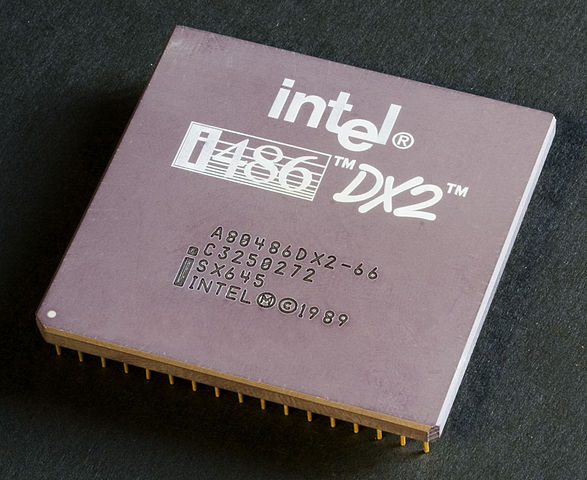
\includegraphics[height=11em]{figs/CPU.jpg}
\hspace{2em}
%https://commons.wikimedia.org/wiki/File:Memory_module_DDRAM_20-03-2006.jpg
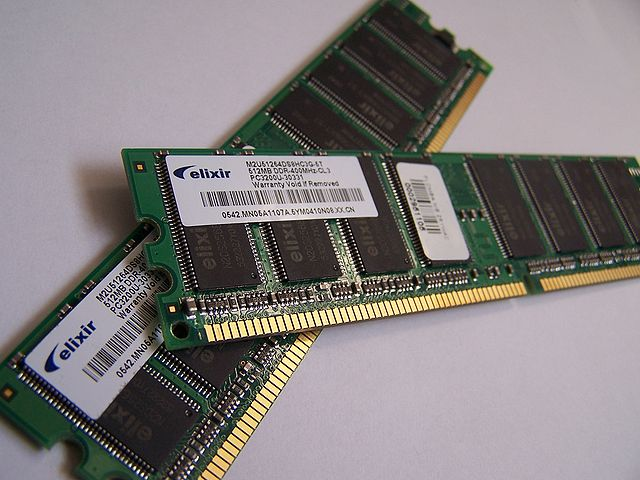
\includegraphics[height=11em]{figs/RAM.jpg}
\caption{Example processor and memory hardware.}
\label{fig.cpuram}
\end{center}
\end{figure}

In 2018 it's common, even for a smartphone, to have four processors and four gigabytes (four billion cells) of memory.
Users generally see and interact with touchscreens, keyboards, and monitors, but it's the processors and memory that perform the actual computations.

When Netflix rents computers from Amazon.com to offer streaming video, what Amazon actually provides is access to server machines that have processors and memory, but no screens or keyboards.

Processors and memory is where computing happens, but they are useless without input/ouput (I/O) devices to receive and send data.
Keyboards and screens are I/O devices, as are the Wifi radios embedded in laptops and smartphones.
Servers like Amazon's have one main I/O device: a network interface which ultimately connects to the laptop where you watch movies.
The Go language was designed primarily to program network connected servers.


\section{What is programming?}

\index{program}

A {\bf program} is a sequence of instructions that specifies how to perform a computation on computer hardware.
The computation might be something mathematical, like solving a system of equations or finding the roots of a polynomial.
It could also be a symbolic computation, like searching and replacing text in a document or (strangely enough) compiling a program.

The details look different in different languages, but a few basic instructions appear in just about every language:

\begin{description}
\item[input:] Get data from the keyboard, a file, the network, a camera, or some other device like a temperature sensor.
\item[output:] Display data on the screen, write it to a file, send it over the network, or activate a device like a door lock.
\item[math:] Perform basic mathematical operations like addition and division.
\item[decisions:] Check for certain conditions and execute the appropriate code.
\item[repetition:] Perform some action repeatedly, usually with some variation.
\end{description}

\index{programming}

Believe it or not, that's pretty much all there is to it.
Every program you've ever used, no matter how complicated, is made up of small instructions that look much like these.
So you can think of {\bf programming} as the process of breaking down a large, complex task into smaller and smaller subtasks.
The process continues until the subtasks are simple enough to be performed with the electronic circuits provided by the hardware.

\section{The hello world program}
\label{hello}

Traditionally, the first program you write when learning a new programming language is called the hello world program.
All it does is display the words ``Hello, World!''\ on the terminal.
In Go, it looks like this:

\index{hello.go}

\begin{lstlisting}
package main

import "fmt"

func main() {
	// display traditional greeting
	fmt.Println("Hello, World!") 
}
\end{lstlisting}

When this program runs it displays:

\begin{stdout}
Hello, World!
\end{stdout}

Notice that the output does not include the quotation marks.


\index{function}
\index{Println function}

Go programs are made up of {\em function} definitions, and functions are made up of {\em statements}.
A {\bf statement} is a line of code that performs a basic action.
The usual way of performing actions is by calling functions that are written by others, such as the Go authors.
So you write functions and your functions, in turn, call other functions.
In the hello world program, this statement calls the {\bf Println} function to display a message on the screen:

\begin{lstlisting}
	fmt.Println("Hello, World!")
\end{lstlisting}

\index{Println}

\java{fmt.Println} displays results on the screen; the name \java{Println} stands for ``print line''.
Confusingly, {\em print} can mean both ``display on the screen'' and ``send to the printer''.
In this book, we'll try to say ``display'' when we mean output to the screen.

\index{case-sensitive}

Go is ``case-sensitive'', which means that uppercase and lowercase are not the same.
In this example, \java{Println} has to begin with an uppercase letter; \java{println} and \java{PRINTLN} won't work.

\index{main function}

A {\bf function} is a sequence of statements.
Functions usually have names, but Go also allows anonymous functions, as we'll see in Chapter XXX.
This code defines a function named \java{main}:

\begin{lstlisting}
func main() {
	// display traditional greeting
	fmt.Println("Hello, World!")
}
\end{lstlisting}

\index{main}

The function name \java{main} is special: when the program runs,
it starts at the first statement in \java{main} and ends when it finishes the last statement.
Later, we will see programs that define more than one function.

\index{\{\} curly braces}
\index{brackets!curly}

Go uses curly braces (\{ and \}) to group things together.
In {\tt hello.go}, the braces contain the body of the function definition.

\index{comment!end-of-line}
\index{statement!comment}

The line that begins with two slashes (\java{//}) is a {\bf comment}, which is a bit of English text that explains the code.
When Go sees \java{//}, it ignores everything from there until the end of the line.
Comments have no effect on the execution of the program, but they make it easier for other programmers (and your future self) to understand what you meant to do.


\index{package}

A {\bf package} is a collection of functions.
The {\tt hello.go} program defines a package named \java{main}. That is also a special name, and it is mandatory for stand-alone programs
--- as opposed to packages designed as parts for larger programs. 

\index{import}

The \java{import} statement declares that our program needs to use the \java{fmt} package, which is part of the Go standard library: a colection of packages providing many ready to use functions. The \java{fmt} name comes from ``format''. The \java{fmt} package has several functions for writing and reading formatted text, such as \java{fmt.Println}.


\section{Compiling Go programs}

\index{high-level language}
\index{language!high-level}

The programming language you will learn in this book is Go, which is a {\bf high-level language}.
Other high-level languages you may have heard of include Java, Python, C, C++, PHP, Ruby, and JavaScript.

\index{machine language}
\index{language!high-level}

Before they can run, programs in high-level languages have to be translated into ``machine language'', the low-level instructions that the computer can follow.
This translation takes some time, which is a small disadvantage of high-level languages.
But high-level languages have two major advantages:

\begin{itemize}

\item It is {\em much} easier to program in a high-level language.
Programs take less time to write, they are shorter and easier to read, and they are more likely to be correct.

\index{portable}

\item High-level languages are {\bf portable}, meaning they can run on different kinds of computers with few or no modifications.
Machine language programs can only run on one kind of computer, and have to be rewritten to run on another.

\end{itemize}

\index{interpret}

Two kinds of programs translate high-level languages into low-level languages: interpreters and compilers.
An {\bf interpreter} reads a high-level program and executes it, meaning that it does what the program says.
It processes the program a little at a time, alternately reading lines and performing computations.
Figure~\ref{fig.interpreter} shows the structure of an interpreter.

\begin{figure}[!ht]
\begin{center}
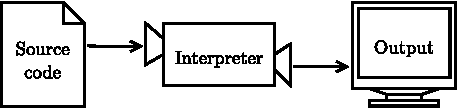
\includegraphics{figs/interpreter.pdf}
\caption{How interpreted languages are executed.}
\label{fig.interpreter}
\end{center}
\end{figure}

\index{compile}
\index{source code}
\index{object code}
\index{executable}

In contrast, a {\bf compiler} reads the entire program and translates it completely before the program starts running.
In this context, the high-level program is called the {\bf source code}, and the translated program is called the {\bf object code} or the {\bf executable}.
Once a program is compiled, you can execute it repeatedly without further translation.
As a result, compiled programs often run faster than interpreted programs.

Figure~\ref{fig.compiler} shows the steps of the development process.
We use the command {\tt go build} to run the Go compile.
It translates {\tt .go} files into binary executable files that store the resulting machine code.
To run the executable, we just call it by name on the command line.

\begin{figure}[!ht]
\begin{center}
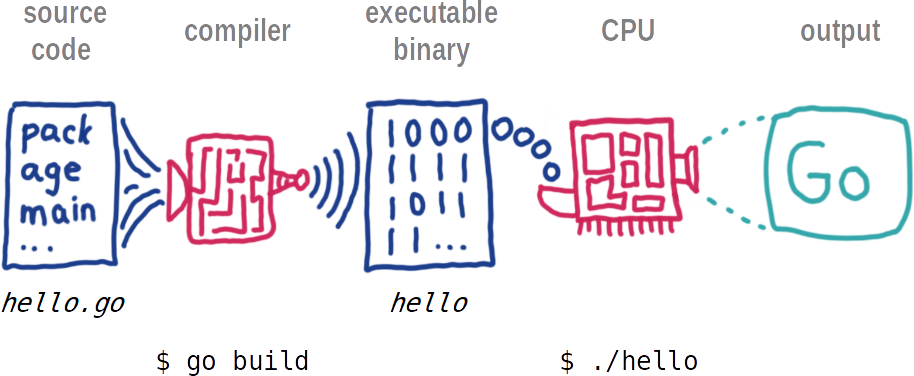
\includegraphics{figs/compiler.png}
\caption{The process of compiling and running a Go program.}
\label{fig.compiler}
\end{center}
\end{figure}

The programmer writes source code in the file {\tt hello.go} and uses {\tt go build} to compile it.
If there are no errors, the compiler saves the executable in the file {\tt hello} (or {\tt hello.exe}, in Windows).
To run the program, the user simply invokes it in the terminal.
The output of the program is then displayed on the screen.

This is how running {\tt hello.go} looks like on the {\tt bash} shell installed by default on GNU/Linux and Mac OS X machines:

\begin{verbatim}
$ ./hello 
Hello, World!
\end{verbatim}

On the Windows command prompt, it's very similar:

\begin{verbatim}
> hello.exe 
Hello, World!
\end{verbatim}


Although it might seem complicated, these steps are automated for you in most program development environments.
Usually you only have to press a button or type a single command to compile and run your program.
On the other hand, it is important to know what steps are happening in the background,
so if something goes wrong you can figure out what it is.


\section{Displaying two messages}

You can put as many statements as you like in the \java{main} method.
For example, to display more than one line of output:

\begin{lstlisting}
package main

import "fmt"

func main() {
	// display traditional greeting
	fmt.Println("Hello, World!") // first line
	fmt.Println("How are you?")  // another line
}
\end{lstlisting}

As this example shows, you can put comments at the end of a line as well as on lines all by themselves.

\index{quote mark}
\index{string}
\index{type!String}
\index{char}

Phrases that appear in quotation marks are called {\bf strings}, because they contain a sequence of characters strung together in memory.
Characters can be letters, ideograms, numbers, punctuation, symbols, spaces, tabs, emojis, etc.

\index{newline}
\index{Println}

\java{fmt.Println} appends a special character, called a {\bf newline}, that breaks the current line and starts a new one.
If you don't want a newline at the end, you can use \java{fmt.Print} instead of \java{fmt.Print}:

\begin{lstlisting}
package main

import "fmt"

func main() {
	fmt.Print("Goodbye, ")
	fmt.Println("cruel world")
}
\end{lstlisting}

\label{goodbye}

In this example, the first statement does not add a newline, so the output appears on a single line as {\tt Goodbye, cruel world}.
Notice that there is a space at the end of the first string, which appears in the output just before the word cruel.


\section{Formatting source code}
\label{formatting}

In Go source code, some spaces are required.
For example, you need at least one space between words, so this program is not legal:

\begin{verbatim}
packagemain

import"fmt"

funcmain() {
	fmt.Println("Hello, World!") 
}
\end{verbatim}


But most other spaces are optional.
For example, this program {\em is} legal:

\begin{lstlisting}
package main
import "fmt"
func main() {
fmt.Println("Hello, World!") 
}
\end{lstlisting}

However, it's harder to read because the structure of the program is not clear.
Tabs and spaces are important for organizing your program visually, making it easier to understand the program and find errors when they occur.

Go also provides a tool, {\tt gofmt}, which rewrites source code in a standard, readable format. Many editors will automatically run {\tt gofmt} when you save a Go source file. 
% LR: similar for VS Code... For example, in DrJava (see Appendix~\ref{drjava}) you can indent your code by selecting all text ({\sf Ctrl+A}) and pressing the {\sf Tab} key.


\section{Escape sequences}

It's possible to display multiple lines of output with only one line of code.
You just have to tell Go where to put the line breaks.

\begin{lstlisting}
package main

import "fmt"

func main() {
	// display traditional greeting
	fmt.Println("Hello!\nHow are you?")
}
\end{lstlisting}

The output is two lines, each ending with a newline character:

\begin{stdout}
Hello!
How are you doing?
\end{stdout}

\index{escape sequence}

The \verb"\n" is an {\bf escape sequence}, or two characters of source code that represent a single character.
(The backslash allows you to ``escape'' the string to write special characters.)
Notice there is no space between \verb"\n" and \verb"How".
If you add a space there, there will be a space at the beginning of the second line.

\begin{table}[!ht]
\begin{center}
\begin{tabular}{|c|c|}
\hline
\verb"\n" & newline \\
\hline
\verb"\t" & tab \\
\hline
\verb'\"' & double quote \\
\hline
\verb"\\" & backslash \\
\hline
\end{tabular}
\caption{Common escape sequences}
\label{tab:escape}
\end{center}
\end{table}

Go has a total of ten escape sequences, and the four most commonly used ones are listed in Table~\ref{tab:escape}.
For example, to write quotation marks inside of strings, you need to escape them with a backslash.

\begin{code}
fmt.Println("She said \"Hello!\" to me.");
\end{code}

The result is:

\begin{stdout}
She said "Hello!" to me.
\end{stdout}

% LR: 2018-01-10: insert ThPy2e "Formal and natural languages" section here
% Drop next section?

\section{What is computer science?}

This book intentionally omits some details about the Go language (such as the other escape sequences),
because our main goal is learning how to think like a computer scientist.
Being able to understand computation is much more valuable than just learning how to write code.

If you're interested in learning more about Go itself, visit the official website: \url{https://golang.org/}.
The interactive tutorial \href{https://tour.golang.org/welcome/1}{\bf A Tour of Go} is a good place to start.

One of the most interesting aspects of writing programs is deciding how to solve a particular problem, especially when there are multiple solutions.
For example, there are numerous ways to sort a list of numbers, and each way has its advantages.
\href{https://www.toptal.com/developers/sorting-algorithms/}{\tt Sorting-algorithms.com} provides animations and descriptions for eight of the most common ways.
In order to determine which way is best for a given situation, we need techniques for describing and analyzing solutions formally.

\index{algorithm}
\index{computer science}

An {\bf algorithm} is a sequence of steps that specifies how to solve a problem.
Some algorithms are faster than others, and some use less space in computer memory.
{\bf Computer science} is the science of algorithms, including their discovery and analysis.
As you learn to develop algorithms for problems you haven't solved before, you will learn to think like a computer scientist.
%It's much more fun to discover new algorithms than to write the code for solutions that other people came up with!

\index{bug}
\index{debugging}

Designing algorithms and writing code is difficult and error-prone.
For historical reasons, programming errors are called {\bf bugs}, and the process of tracking them down and correcting them is called {\bf debugging}.
As you learn to debug your programs, you will develop new problem-solving skills.
You will need to think creatively when unexpected errors happen.

Although it can be frustrating, debugging is an intellectually rich, challenging, and interesting part of computer science.
In some ways, debugging is like detective work.
You are confronted with clues, and you have to infer the processes and events that led to the results you see.
Thinking about how to correct programs and improve their performance sometimes even leads to the discovery of new algorithms.


\section{Debugging programs}
\label{sec:examples}

It is a good idea to read this book in front of a computer so you can try out the examples as you go.
You can run many of the examples directly in DrJava's Interactions Pane (see Appendix~\ref{interactions}).
But if you put the code in a source file, it will be easier to try out variations.

\index{error!message}

Whenever you are experimenting with a new feature, you should also try to make mistakes.
For example, in the hello world program, what happens if you leave out one of the quotation marks?
What if you leave out both?
What if you spell \java{println} wrong?
These kinds of experiments help you remember what you read.
They also help with debugging, because you learn what the error messages mean.
It is better to make mistakes now and on purpose than later on and accidentally.

\index{experimental debugging}
\index{debugging!experimental}

%\index{Holmes, Sherlock}
%\index{Doyle, Arthur Conan}

Debugging is like an experimental science: once you have an idea about what is going wrong, you modify your program and try again.
If your hypothesis was correct, then you can predict the result of the modification, and you take a step closer to a working program.
If your hypothesis was wrong, you have to come up with a new one.
%As Sherlock Holmes pointed out, ``When you have eliminated the impossible, whatever remains, however improbable, must be the truth.''
%(A.~Conan Doyle, {\em The Sign of Four}.)

Programming and debugging should go hand in hand.
Don't just write a bunch of code and then perform trial and error debugging until it all works.
Instead, start with a program that does {\em something} and make small modifications, debugging them as you go, until the program does what you want.
That way you will always have a working program, and it will be easier to isolate errors.

\index{Linux}
\index{Torvalds, Linus}
\index{Greenfield, Larry}

A great example of this principle is the Linux operating system, which contains millions of lines of code.
It started out as a simple program Linus Torvalds used to explore the Intel 80386 chip.
According to Larry Greenfield in {\it The Linux Users' Guide}, ``One of Linus's earlier projects was a program that would switch between printing AAAA and BBBB.
This later evolved to Linux.''

%Later chapters will make more suggestions about debugging and other programming practices.

Finally, programming sometimes brings out strong emotions.
If you are struggling with a difficult bug, you might feel angry, despondent, or embarrassed.
Remember that you are not alone, and virtually every programmer has had similar experiences.
Don't hesitate to reach out to a friend and ask questions!

%That's why this chapter is called, ``The way of the program''.


\section{Vocabulary}

Throughout the book, we try to define each term the first time we use it.
At the end of each chapter, we include the new terms and their definitions in order of appearance.
If you spend some time learning this vocabulary, you will have an easier time reading the following chapters.

\begin{description}

\term{problem solving}
The process of formulating a problem, finding a solution, and expressing the solution.

\term{hardware}
The electronic and mechanical components of a computer, such as CPUs, RAM, and hard disks.

\term{processor}
A computer chip that performs simple instructions like basic arithmetic and logic.

\term{memory}
Circuits that store data as long as the computer is turn on.
Not to be confused with permanent storage devices like hard disks and flash.

\term{program}
A sequence of instructions that specifies how to perform tasks on a computer.
Also known as software.

\term{programming}
The application of problem solving to creating executable computer programs.

\term{statement}
Part of a program that specifies one step of an algorithm.

\term{print statement}
A statement that causes output to be displayed on the screen.

\term{method}
A named sequence of statements.

\term{class}
For now, a collection of related methods.
(We will see later that there is a lot more to it.)

\term{comment}
A part of a program that contains information about the program but has no effect when the program runs.

\term{high-level language}
A programming language that is designed to be easy for humans to read and write.

\term{low-level language}
A programming language that is designed to be easy for a computer to run.
Also called ``machine language'' or ``assembly language''.

\term{portable}
The ability of a program to run on more than one kind of computer.

\term{interpret}
To run a program in a high-level language by translating it one line at a time and immediately executing the corresponding instructions.

\term{compile}
To translate a program in a high-level language into a low-level language, all at once, in preparation for later execution.

\term{source code}
A program in a high-level language, before being compiled.

\term{object code}
The output of the compiler, after translating the program.

\term{executable}
Another name for object code that is ready to run on specific hardware.

\term{byte code}
A special kind of object code used for Java programs.
Byte code is similar to a low-level language, but it is portable like a high-level language.

\term{string}
A sequence of characters; the primary data type for text.

\term{newline}
A special character signifying the end of a line of text.
Also known as line ending, end of line (EOL), or line break.

%\term{whitespace}
%Newlines, tab characters, and other spaces in a source program.
%Whitespace characters are used to separate words, but other than that, they don't affect the behavior of the program.

\term{escape sequence}
A sequence of code that represents a special character when used inside a string.

\term{algorithm}
A procedure or formula for solving a problem, with or without a computer.

\term{computer science}
The scientific and practical approach to computation and its applications.

\term{bug}
An error in a program.

\term{debugging}
The process of finding and removing errors.

\end{description}


\section{Exercises}

At the end of each chapter, we include exercises you can do with the things you've learned.
We encourage you to at least attempt every problem.
You can't learn to program only by reading about it; you have to practice.

Before you can compile and run Java programs, you might have to download and install a few tools.
There are many good options, but we recommend DrJava, which is an ``integrated development environment'' (IDE) well suited for beginners.
Instructions for getting started are in Appendix~\ref{tools}.

The code for this chapter is in the {\tt ch01} directory of {\tt ThinkJavaCode2}.
See page~\pageref{code} for instructions on how to download the repository.
Before you start the exercises, we recommend that you compile and run the examples.


\begin{exercise}  %%V6 Ex1.1

Computer scientists have the annoying habit of using common English words to mean something other than their common English meaning.
For example, in English, statements and comments are the same thing, but in programs they are different.

\begin{enumerate}
\item In computer jargon, what's the difference between a statement and a comment?
\item What does it mean to say that a program is portable?
\item In common English, what does the word compile mean?
\item What is an executable? Why is that word used as a noun?
\end{enumerate}

The glossary at the end of each chapter is intended to highlight words and phrases that have special meanings in computer science.
When you see familiar words, don't assume that you know what they mean!

\end{exercise}


\begin{exercise}  %%V6 Ex1.2

Before you do anything else, find out how to compile and run a Java program.
Some environments provide sample programs similar to the example in Section~\ref{hello}.

\begin{enumerate}
\item Type in the hello world program, then compile and run it.

\item Add a print statement that displays a second message after the ``Hello, World!''.
Say something witty like, ``How are you?''
Compile and run the program again.

\item Add a comment to the program (anywhere), recompile, and run it again.
The new comment should not affect the result.
\end{enumerate}

This exercise may seem trivial, but it is the starting place for many of the programs we will work with.
To debug with confidence, you will need to have confidence in your programming environment.

In some environments, it is easy to lose track of which program is executing.
You might find yourself trying to debug one program while you are accidentally running another.
Adding (and changing) print statements is a simple way to be sure that the program you are looking at is the program you are running.

\end{exercise}


\begin{exercise}  %%V6 Ex1.3

It is a good idea to commit as many errors as you can think of, so that you see what error messages the compiler produces.
Sometimes the compiler tells you exactly what is wrong, and all you have to do is fix it.
But sometimes the error messages are misleading.
Over time you will develop a sense for when you can trust the compiler and when you have to figure things out yourself.

Starting with the hello world program, try out each of the following errors.
After you make each change, compile the program, read the error message (if there is one), and then fix the error.

\begin{enumerate}
\item Remove one of the open curly braces.
\item Remove one of the close curly braces.
\item Instead of \java{main}, write \java{mian}.
\item Remove the word \java{static}.
\item Remove the word \java{public}.
\item Remove the word \java{System}.
\item Replace \java{println} with \java{Println}.
\item Replace \java{println} with \java{print}.
\item Delete one of the parentheses.
\item Add an extra parenthesis.
\end{enumerate}

\end{exercise}



\appendix
\addtocontents{toc}{\protect\newpage}

%BEGIN LATEX
\renewcommand{\chaptermark}[1]{\markboth{Appendix \thechapter ~~ #1}{}}
%END LATEX

\chapter{Debugging}
\label{debugging}

\index{debugging}

Although there are debugging suggestions throughout the book, we thought it would be useful to organize them in an appendix.
If you are having a hard time debugging, you might want to review this appendix from time to time.

The best debugging strategy depends on what kind of error you have:

\begin{itemize}

\item {\bf Compile-time errors} indicate that there is something wrong with the syntax of the program.
Example: omitting the semicolon at the end of a statement.

\index{compile-time error}
\index{error!compile-time}
\index{syntax}

\item {\bf Run-time errors} are produced if something goes wrong while the program is running.
Example: an infinite recursion eventually causes a \java{StackOverflowError}.

\index{run-time error}
\index{error!run-time}
\index{exception}

\item {\bf Logic errors} cause the program to do the wrong thing.
Example: an expression may not be evaluated in the order you expect.

\index{logic error}
\index{error!logic}

\end{itemize}

The following sections are organized by error type; some techniques are useful for more than one type.


\section{Compile-time errors}

The best kind of debugging is the kind you don't have to do because you avoid making errors in the first place.
Incremental development, which we presented in Section~\ref{distance}, can help.
The key is to start with a working program and add small amounts of code at a time.
When there is an error, you will have a pretty good idea where it is.

Nevertheless, you might find yourself in one of the following situations.
For each situation, we have some suggestions about how to proceed.


\subsection*{The compiler is spewing error messages.}

\index{compile}
\index{error!message}

If the compiler reports 100 error messages, that doesn't mean there are 100 errors in your program.
When the compiler encounters an error, it often gets thrown off track for a while.
It tries to recover and pick up again after the first error, but sometimes it reports spurious errors.

Only the first error message is truly reliable.
We suggest that you only fix one error at a time, and then recompile the program.
You may find that one semicolon or brace ``fixes'' 100 errors.


\subsection*{I'm getting a weird compiler message, and it won't go away.}

First of all, read the error message carefully.
It may be written in terse jargon, but often there is a carefully hidden kernel of information.

If nothing else, the message will tell you where in the program the problem occurred.
Actually, it tells you where the compiler was when it noticed a problem, which is not necessarily where the error is.
Use the information the compiler gives you as a guideline, but if you don't see an error where the compiler is pointing, broaden the search.

Generally the error will be prior to the location of the error message, but there are cases where it will be somewhere else entirely.
For example, if you get an error message at a method invocation, the actual error may be in the method definition itself.

If you don't find the error quickly, take a breath and look more broadly at the entire program.
Make sure the program is indented properly; that makes it easier to spot syntax errors.

Now, start looking for common syntax errors:

\index{syntax errors}
\index{error!syntax}

\begin{enumerate}

\item Check that all parentheses and brackets are balanced and properly nested.
All method definitions should be nested within a class definition.
All program statements should be within a method definition.

\item Remember that uppercase letters are not the same as lowercase letters.

\item Check for semicolons at the end of statements (and no semicolons after curly braces).

\index{quote mark}

\item Make sure that any strings in the code have matching quotation marks.
Make sure that you use double quotes for strings and single quotes for characters.

\item For each assignment statement, make sure that the type on the left is the same as the type on the right.
Make sure that the expression on the left is a variable name or something else that you can assign a value to (like an element of an array).

\item For each method invocation, make sure that the arguments you provide are in the right order and have the right type, and that the object you are invoking the method on is the right type.

\item If you are invoking a value method, make sure you are doing something with the result.
If you are invoking a void method, make sure you are {\em not} trying to do something with the result.

\item If you are invoking an instance method, make sure you are invoking it on an object with the right type.
If you are invoking a static method from outside the class where it is defined, make sure you specify the class name (using dot notation).

\item Inside an instance method you can refer to the instance variables without specifying an object.
If you try that in a static method -- with or without \java{this} -- you get a message like ``non-static variable x cannot be referenced from a static context.''

\end{enumerate}

If nothing works, move on to the next section...


\subsection*{I can't get my program to compile no matter what I do.}

If the compiler says there is an error and you don't see it, that might be because you and the compiler are not looking at the same code.
Check your development environment to make sure the program you are editing is the program the compiler is compiling.

This situation is often the result of having multiple copies of the same program.
You might be editing one version of the file, but compiling a different version.

If you are not sure, try putting an obvious and deliberate syntax error right at the beginning of the program.
Now compile again.
If the compiler doesn't find the new error, there is probably something wrong with the way you set up the development environment.

\index{debugging!by bisection}

If you have examined the code thoroughly, and you are sure the compiler is compiling the right source file, it is time for desperate measures: {\bf debugging by bisection}.

\begin{itemize}

\item Make a backup of the file you are working on.
If you are working on {\tt Bob.java}, make a copy called {\tt Bob.java.old}.

\item Delete about half the code from {\tt Bob.java}.
Try compiling again.

\begin{itemize}

\item If the program compiles now, you know the error is in the code you deleted.
Bring back about half of what you deleted and repeat.

\item If the program still doesn't compile, the error must be in the code that remains.
Delete about half of the remaining code and repeat.

\end{itemize}

\item Once you have found and fixed the error, start bringing back the code you deleted, a little bit at a time.

\end{itemize}

This process is ugly, but it goes faster than you might think, and it is very reliable.
It works for other programming languages too!


\subsection*{I did what the compiler told me to do, but it still doesn't work.}

Some error messages come with tidbits of advice, like ``class Golfer must be declared abstract.
It does not define int compareTo(java.lang.Object) from interface java.lang.Comparable.''
It sounds like the compiler is telling you to declare \java{Golfer} as an \java{abstract} class, and if you are reading this book, you probably don't know what that is or how to do it.

Fortunately, the compiler is wrong.
The solution in this case is to make sure \java{Golfer} has a method called \java{compareTo} that takes an \java{Object} as a parameter.

Don't let the compiler lead you by the nose.
Error messages give you evidence that something is wrong, but the remedies they suggest are unreliable.


\section{Run-time errors}

It's not always clear what causes a run-time error, but you can often figure things out by adding print statements to your program.


\subsection*{My program hangs.}

\index{hanging}
\index{infinite loop}
\index{infinite recursion}

If a program stops and seems to be doing nothing, we say it is ``hanging''.
Often that means it is caught in an infinite loop or an infinite recursion.

\begin{itemize}

\item If there is a particular loop that you suspect is the problem, add a print statement immediately before the loop that says ``entering the loop'' and another immediately after that says ``exiting the loop''.

Run the program.
If you get the first message and not the second, you know where the program is getting stuck.
Go to the section titled ``Infinite loop''.% on page~\pageref{infloop}.

\index{StackOverflowError}

\item Most of the time an infinite recursion will cause the program to run for a while and then produce a \java{StackOverflowError}.
If that happens, go to the section titled ``Infinite recursion''.% on page~\pageref{infrec}.

If you are not getting a \java{StackOverflowError}, but you suspect there is a problem with a recursive method, you can still use the techniques in the infinite recursion section.

\item If neither of the previous suggestions helps, you might not understand the flow of execution in your program.
Go to the section titled ``Flow of execution''.% on page~\pageref{flowexec}.

\end{itemize}


\subsubsection*{Infinite loop}
\label{infloop}

If you think you have an infinite loop and you know which loop it is, add a print statement at the end of the loop that displays the values of the variables in the condition, and the value of the condition.

For example:

\begin{code}
while (x > 0 && y < 0) {
    // do something to x
    // do something to y

    System.out.println("x: " + x);
    System.out.println("y: " + y);
    System.out.println("condition: " + (x > 0 && y < 0));
}
\end{code}

Now when you run the program you see three lines of output for each time through the loop.
The last time through the loop, the condition should be \java{false}.
If the loop keeps going, you will see the values of \java{x} and \java{y}, and you might figure out why they are not getting updated correctly.


\subsubsection*{Infinite recursion}
\label{infrec}

\index{recursion!infinite}
\index{infinite recursion}

Most of the time, an infinite recursion will cause the program to throw a \java{StackOverflowError}.
But if the program is slow, it may take a long time to fill the stack.

If you know which method is causing an infinite recursion, check that there is a base case.
There should be some condition that makes the method return without making a recursive invocation.
If not, you need to rethink the algorithm and identify a base case.

If there is a base case, but the program doesn't seem to be reaching it, add a print statement at the beginning of the method that displays the parameters.
Now when you run the program you see a few lines of output every time the method is invoked, and you can see the values of the parameters.
If the parameters are not moving toward the base case, you might see why not.


\subsubsection*{Flow of execution}
\label{flowexec}

\index{flow of execution}
\index{tracing}

If you are not sure how the flow of execution is moving through your program, add print statements to the beginning of each method with a message like ``entering method foo'', where \java{foo} is the name of the method.
Now when you run the program, it displays a trace of each method as it is invoked.

You can also display the arguments each method receives.
When you run the program, check whether the values are reasonable, and check for one of the most common errors -- providing arguments in the wrong order.


\subsection*{When I run the program I get an exception.}

\index{exception}
\index{stack trace}

When an exception occurs, Java displays a message that includes the name of the exception, the line of the program where the exception occurred, and a ``stack trace''.
The stack trace includes the method that was running, the method that invoked it, the method that invoked that one, and so on.

The first step is to examine the place in the program where the error occurred and see if you can figure out what happened.

\begin{description}

\term{NullPointerException}
You tried to access an instance variable or invoke a method on an object that is currently \java{null}.
You should figure out which variable is \java{null} and then figure out how it got to be that way.

Remember that when you declare a variable with an array type, its elements are initially \java{null} until you assign a value to them.
For example, this code causes a \java{NullPointerException}:

\begin{code}
int[] array = new Point[5];
System.out.println(array[0].x);
\end{code}

\term{ArrayIndexOutOfBoundsException}
The index you are using to access an array is either negative or greater than \java{array.length - 1}.
If you can find the site where the problem is, add a print statement immediately before it to display the value of the index and the length of the array.
Is the array the right size?
Is the index the right value?

Now work your way backwards through the program and see where the array and the index come from.
Find the nearest assignment statement and see if it is doing the right thing.
If either one is a parameter, go to the place where the method is invoked and see where the values are coming from.

\term{StackOverflowError}
See ``Infinite recursion'' on page~\pageref{infrec}.

\term{FileNotFoundException}
This means Java didn't find the file it was looking for.
If you are using a project-based development environment like Eclipse, you might have to import the file into the project.
Otherwise make sure the file exists and that the path is correct.
This problem depends on your file system, so it can be hard to track down.

\term{ArithmeticException}
Something went wrong during an arithmetic operation; for example, division by zero.

\end{description}


\subsection*{I added so many print statements I get inundated with output.}

\index{print statement}
\index{statement!print}

One of the problems with using print statements for debugging is that you can end up buried in output.
There are two ways to proceed: either simplify the output, or simplify the program.

To simplify the output, you can remove or comment out print statements that aren't helping, or combine them, or format the output so it is easier to understand.
As you develop a program, you should write code to generate concise, informative traces of what the program is doing.

To simplify the program, scale down the problem the program is working on.
For example, if you are sorting an array, sort a {\em small} array.
If the program takes input from the user, give it the simplest input that causes the error.

\index{nested}

Also, clean up the code.
Remove unnecessary or experimental parts, and reorganize the program to make it easier to read.
For example, if you suspect that the error is in a deeply-nested part of the program, rewrite that part with a simpler structure.
If you suspect a large method, split it into smaller methods and test them separately.

The process of finding the minimal test case often leads you to the bug.
For example, if you find that a program works when the array has an even number of elements, but not when it has an odd number, that gives you a clue about what is going on.

Reorganizing the program can help you find subtle bugs.
If you make a change that you think doesn't affect the program, and it does, that can tip you off.


\section{Logic errors}


\subsection*{My program doesn't work.}

Logic errors are hard to find because the compiler and interpreter provide no information about what is wrong.
Only you know what the program is supposed to do, and only you know that it isn't doing it.

The first step is to make a connection between the code and the behavior you get.
You need a hypothesis about what the program is actually doing.
Here are some questions to ask yourself:

\begin{itemize}

\item Is there something the program was supposed to do, but doesn't seem to be happening?
Find the section of the code that performs that function, and make sure it is executing when you think it should.
See ``Flow of execution'' on page~\pageref{flowexec}.

\item Is something happening that shouldn't?
Find code in your program that performs that function, and see if it is executing when it shouldn't.

\item Is a section of code producing an unexpected effect?
Make sure you understand the code, especially if it invokes methods in the Java library.
Read the documentation for those methods, and try them out with simple test cases.
They might not do what you think they do.

\end{itemize}

To program, you need a mental model of what your code does.
If it doesn't do what you expect, the problem might not actually be the program; it might be in your head.

\index{mental model}

The best way to correct your mental model is to break the program into components (usually the classes and methods) and test them independently.
Once you find the discrepancy between your model and reality, you can solve the problem.

Here are some common logic errors to check for:

\index{logic error}
\index{error!logic}

\begin{itemize}

\item Remember that integer division always rounds toward zero.
If you want fractions, use \java{double}.
More generally, use integers for countable things and floating-point numbers for measurable things.

\item Floating-point numbers are only approximate, so don't rely on them to be perfectly accurate.
You should probably never use the \java{==} operator with \java{double}s.
Instead of writing \java{if (d == 1.23)}, do something like \java{if (Math.abs(d - 1.23) < .000001)}.

% NOTE: should not be possible in Java, because = can't be used in a boolean expression
%\item If you use the assignment operator (\java{=}) instead of the equality operator (\java{==}) in the condition of an \java{if}, \java{while}, or \java{for} statement, you might get an expression that is syntactically legal and logically wrong.

\item When you apply the equality operator (\java{==}) to objects, it checks whether they are identical.
If you meant to check equivalence, you should use the \java{equals} method instead.

\item By default for user-defined types, \java{equals} checks identity.
If you want a different notion of equivalence, you have to override it.

\item Inheritance can lead to subtle logic errors, because you can run inherited code without realizing it.
See ``Flow of execution'' on page~\pageref{flowexec}.

\end{itemize}


\subsection*{I've got a big hairy expression and it doesn't do what I expect.}

\index{expression!big and hairy}

Writing complex expressions is fine as long as they are readable, but they can be hard to debug.
It is often a good idea to break a complex expression into a series of assignments to temporary variables.

\begin{code}
rect.setLocation(rect.getLocation().translate(
                 -rect.getWidth(), -rect.getHeight()));
\end{code}

This example can be rewritten as:

\begin{code}
int dx = -rect.getWidth();
int dy = -rect.getHeight();
Point location = rect.getLocation();
Point newLocation = location.translate(dx, dy);
rect.setLocation(newLocation);
\end{code}

The second version is easier to read, partly because the variable names provide additional documentation.
It's also easier to debug, because you can check the types of the temporary variables and display their values.

\index{temporary variable}
\index{variable!temporary}
\index{order of operations}
\index{precedence}

Another problem that can occur with big expressions is that the order of operations may not be what you expect.
For example, to evaluate $\frac{x}{2 \pi}$, you might write:

\begin{code}
double y = x / 2 * Math.PI;
\end{code}

That is not correct, because multiplication and division have the same precedence, and they are evaluated from left to right.
This code computes $\frac{x}{2}\pi$.

If you are not sure of the order of operations, check the documentation, or use parentheses to make it explicit.

\begin{code}
double y = x / (2 * Math.PI);
\end{code}

This version is correct, and more readable for other people who haven't memorized the order of operations.


\subsection*{My method doesn't return what I expect.}

\index{return statement}
\index{statement!return}

If you have a return statement with a complex expression, you don't have a chance to display the value before returning.

\begin{code}
public Rectangle intersection(Rectangle a, Rectangle b) {
    return new Rectangle(
        Math.min(a.x, b.x), Math.min(a.y, b.y),
        Math.max(a.x + a.width, b.x + b.width)
            - Math.min(a.x, b.x)
        Math.max(a.y + a.height, b.y + b.height)
            - Math.min(a.y, b.y));
}
\end{code}

Instead of writing everything in one statement, use temporary variables:

\begin{code}
public Rectangle intersection(Rectangle a, Rectangle b) {
    int x1 = Math.min(a.x, b.x);
    int y1 = Math.min(a.y, b.y);
    int x2 = Math.max(a.x + a.width, b.x + b.width);
    int y2 = Math.max(a.y + a.height, b.y + b.height);
    Rectangle rect = new Rectangle(x1, y1, x2 - x1, y2 - y1);
    return rect;
}
\end{code}

Now you have the opportunity to display any of the intermediate variables before returning.
And by reusing \java{x1} and \java{y1}, you made the code smaller, too.


\subsection*{My print statement isn't doing anything.}

\index{print statement}
\index{statement!print}

If you use the \java{println} method, the output is displayed immediately, but if you use \java{print} (at least in some environments), the output gets stored without being displayed until the next newline.
If the program terminates without displaying a newline, you may never see the stored output.
If you suspect that this is happening, change some or all of the \java{print} statements to \java{println}.


\subsection*{I'm really, really stuck and I need help.}

First, get away from the computer for a few minutes.
Computers emit waves that affect the brain, causing the following symptoms:

\begin{itemize}

\item Frustration and rage.

\item Superstitious beliefs (``the computer hates me'') and magical thinking (``the program only works when I wear my hat backwards'').

\item Sour grapes (``this program is lame anyway'').

\end{itemize}

If you suffer from any of these symptoms, get up and go for a walk.
When you are calm, think about the program.
What is it doing?
What are possible causes of that behavior?
When was the last time you had a working program, and what did you do next?

Sometimes it just takes time to find a bug.
People often find bugs when they let their mind wander.
Good places to find bugs are buses, showers, and bed.


\subsection*{No, I really need help.}

It happens.
Even the best programmers get stuck.
Sometimes you need another pair of eyes.

Before you bring someone else in, make sure you have tried the techniques described in this appendix.

Your program should be as simple as possible, and you should be working on the smallest input that causes the error.
You should have print statements in the appropriate places (and the output they produce should be comprehensible).
You should understand the problem well enough to describe it concisely.

When you bring someone in to help, give them the information they need:

\begin{itemize}

\item What kind of bug is it?
Compile-time, run-time, or logic?

\item What was the last thing you did before this error occurred?
What were the last lines of code that you wrote, or what is the test case that fails?

\item If the bug occurs at compile time or run time, what is the error message, and what part of the program does it indicate?

\item What have you tried, and what have you learned?

\end{itemize}

By the time you explain the problem to someone, you might see the answer.
This phenomenon is so common that some people recommend a debugging technique called ``rubber ducking''.
Here's how it works:

\index{rubber duck}
\index{debugging!rubber duck}

\begin{enumerate}

\item Buy a standard-issue rubber duck.

\item When you are really stuck on a problem, put the rubber duck on the desk in front of you and say, ``Rubber duck, I am stuck on a problem.
Here's what's happening...''

\item Explain the problem to the rubber duck.

\item Discover the solution.

\item Thank the rubber duck.

\end{enumerate}

We're not kidding, it works!
See \url{https://en.wikipedia.org/wiki/Rubber_duck_debugging}.


\subsection*{I found the bug!}

When you find the bug, it is usually obvious how to fix it.
But not always.
Sometimes what seems to be a bug is really an indication that you don't understand the program, or there is an error in your algorithm.
In these cases, you might have to rethink the algorithm, or adjust your mental model.
Take some time away from the computer to think, work through test cases by hand, or draw diagrams to represent the computation.

After you fix the bug, don't just start in making new errors.
Take a minute to think about what kind of bug it was, why you made the error, how the error manifested itself, and what you could have done to find it faster.
Next time you see something similar, you will be able to find the bug more quickly.
Or even better, you will learn to avoid that type of bug for good.



\backmatter

\printindex

%-------------------------------------------------------------
\newpage
\thispagestyle{empty}

\vspace*{64pt}

{\bf\huge About the Authors}

\vspace*{40pt}

{\bf Luciano Ramalho} is the author of Fluent Python (O'Reilly, 2015) and a principal consultant at ThoughtWorks.
He is a self-taught programmer who's been teaching programming languages to beginners and professionals since 1984.

{\bf Allen Downey} is a Professor of Computer Science at Olin College of Engineering.
He has taught computer science at Wellesley College, Colby College, and U.C. Berkeley.
He has a Ph.D. in Computer Science from U.C. Berkeley and Master's and Bachelor's degrees from MIT.

{\bf Chris Mayfield} is an Associate Professor of Computer Science at James Madison University, with a research focus on CS education and professional development.
He has a Ph.D. in Computer Science from Purdue University and Bachelor's degrees in CS and German from the University of Utah.

\end{document}
